\documentclass[14pt]{beamer}
\usepackage[T2A]{fontenc}
\usepackage[utf8]{inputenc}
\usepackage[english]{babel}
\usepackage{amssymb,amsfonts,amsmath,mathtext}
\usepackage{cite,enumerate,float,indentfirst}

\usepackage{multicol}
\usepackage{listings}

\graphicspath{{images/}}

\usetheme{Pittsburgh}
\usecolortheme{whale}

\setlength{\columnseprule}{1pt}
\def\columnseprulecolor{\color{blue}}

\setbeamercolor{footline}{fg=blue}
\setbeamertemplate{footline}{
  \leavevmode%
  \hbox{%
  \begin{beamercolorbox}[wd=.333333\paperwidth,ht=2.25ex,dp=1ex,center]{}%
    Boris Kudryashov, ITMO University
  \end{beamercolorbox}%
  \begin{beamercolorbox}[wd=.333333\paperwidth,ht=2.25ex,dp=1ex,center]{}%
    St. Petersburg, 2016
  \end{beamercolorbox}%
  \begin{beamercolorbox}[wd=.333333\paperwidth,ht=2.25ex,dp=1ex,right]{}%
  Page \insertframenumber{} of \inserttotalframenumber \hspace*{2ex}
  \end{beamercolorbox}}%
  \vskip0pt%
}

\newcommand{\itemi}{\item[\checkmark]}

\title{\small{Information Theory. 5th Chapter Slides}}
\author{\huge{
Boris Kudryashov \\
\vspace{30pt}
ITMO University
}}

% \hyperlink{refthis}{here}
% \hypertarget{refthis}{}


\begin{document}

\maketitle



\begin{frame}
\frametitle{Agenda}
\begin{enumerate}
% \footnotesize {
\small{
    \item{Noiseless coding problem statement}
    \item{Channel models}
    \item{Mutual information. Average mutual information}
    \item{Conditional average mutual information. Information rework theorem}
    \item{Convexity of average mutual information}
    \item{Information capacity and throughput}
    \item{Fano inequality}
    \item{Reverse coding theorem}
    \item{Information capacity of memoryless channels}
    \item{Symmetrical channels}
}

\end{enumerate}
\end{frame}


\begin{frame}
\frametitle{Noiseless coding problem statement}
\begin{itemize}

% \footnotesize {
% \small{
    \item $X=\{0, 1\}. Y = X$
    \item Discrete channel with noise.
    \item Develop a code to eliminate errors.


    \pause
    \begin{table}[htbp]
    \begin{center}
    \caption{Example 1}
    \begin{tabular}
        {|c|c|c|} \hline %
        Message & Codeword & Decisive area \\ \hline %
        0& 000&   {\{}000, 001, 010, 100{\}} \\ \hline %
        1& 111&   {\{}011, 101, 110, 111{\}} \\ \hline %
    \end{tabular}
    \end{center}
    \end{table}


% }
\end{itemize}
\end{frame}



\begin{frame}
\frametitle{Noiseless coding problem statement}

% \footnotesize {
% \small{


    \begin{table}[htbp]
    \begin{center}
    \caption{Example 2}
    \begin{tabular}
        {|c|c|c|} \hline %
        Message & Codeword & Decisive area \\ \hline %
        00& 00000& \{00000,00001,00010,00100,  \\
          &      &   01000,10000,11000,10001\} \\  \hline %
        01& 10110& \{10110,10111,10100,10010, \\
          &      &   11110,00110,01110,00111\} \\  \hline %
        10& 01011& \{01011,01010,01001,01111,  \\
          &      &   00011,11011,10011,11010\} \\  \hline %
        11& 11101& \{11101,11100,11111,11001,  \\
          &      &   10101,01101,00101,01100\} \\ \hline %
    \end{tabular}
    \end{center}
    \end{table}

\end{frame}



\begin{frame}
\frametitle{Noiseless coding problem statement}
\begin{itemize}
% \footnotesize {
\small{

    \item
        \begin{figure}[ht]
        \begin{minipage}{1.0\linewidth}
        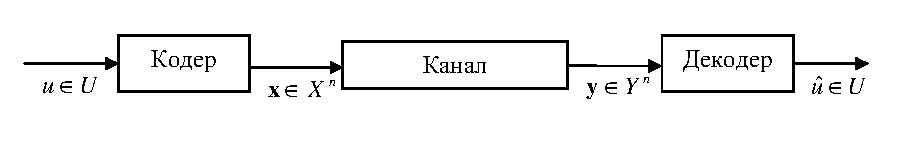
\includegraphics[width=1.0\textwidth]{fig5_1.eps}
        %\centerline{\includegraphics[width=3.16in,height=4.02in]
        \caption{Communication system Scheme}
        \label{fig5_1}
        \end{minipage}
        \end{figure}

    \pause
    \item
        \textit{Code of channel} over $X$ is arbitrary set of sequences $A = \{{\vec x}_m \}$, $m = 1,...,M$, $A \in X^n$.
    \item
        These sequences are \textit{codewords}.
    \item
        Their length $n$ is \textit{code length}.
    \item
        Number of sequences $M$ is \textit{code cardinality}.
        $R$, defined as:
        \begin{equation}
            R = \frac{\log M}{n}
        \end{equation}
        is called \textit{code rate} (bits per symbol).
    \item
        Event when $\hat {u} \ne u$ is \textit{decoding error}.
    \item
        And it's probability is \textit{error probability}
}
\end{itemize}
\end{frame}


% --------------------Channel models----------

\begin{frame}
\frametitle{Channel models}
\begin{itemize}
% \footnotesize {
% \small{
\item
    \textit{Channel model} is defined, if $\forall  n$ and $\forall  {\vec x} \in X^n$, ${\vec y} \in Y^n$ conditional probability $p({\vec y}\vert {\vec x})$ is defined.

\pause \item
    Reminder: ${\vec x}_i^n = (x_i ,...,x_n )$.
    Channel is called \textit{stationary}, if $\forall  j, n $ and $ \forall {\vec x}_{j + 1}^{j + n} \in X^n$, ${\vec y}_{j + 1}^{j + n} \in Y^n$ conditional probabilities $p({\vec y}_{j + 1}^{j + n} \vert {\vec x}_{j + 1}^{j + n} )$ are defined by sequence characters and do not depend from index $j$.

\end{itemize}
\end{frame}


\begin{frame}
\frametitle{Channel models}
\begin{itemize}

\item
Channel is called \textit{memoryless}, if $\forall j,n $ and $\forall {\vec x}_{j + 1}^{j + n} \in X^n$, ${\vec y}_{j + 1}^{j
+ n} \in Y^n$
\[
p({\vec y}_{j + 1}^{j + n} \vert {\vec x}_{j + 1}^{j + n} ) =
\prod\limits_{i = j + 1}^{j + n} {p(y_i \vert x_i )} .
\]


\pause \item
Stationary channel without memory is called discrete stationary channel.

\end{itemize}
\end{frame}


\begin{frame}
\frametitle{Channel models}
\begin{itemize}
% \footnotesize {
% \small{
To describe a Discrete Stationary Channel it's enough to define conditional probabilities $\{p(y\vert x),x \in X,y \in Y\}$. Let $X = \{0,...,K - 1\}$, $Y = \{0,...,L - 1\}$. Let $p_{ij} = p(y = j\vert x = i\}$, $i \in X$, $j \in Y$.
Describe transition probabilities of channel $p_{ij} $ in a \textit{transition probability matrix}:
\[
\left[
  \begin{array}{cccc}
    p_{00} & p_{01} & \cdots & p_{0,L - 1} \\
    p_{10} & p_{11} & \cdots & p_{1,L - 1} \\
    \vdots & \vdots & \ddots & \vdots \\
    p_{K - 1,0} & p_{K - 1,1} & \cdots & p_{K - 1,L - 1} \\
  \end{array}
\right].
\]

\end{itemize}
\end{frame}


\begin{frame}
\frametitle{Channel models}
\begin{itemize}
% \footnotesize {
% \small{

\begin{figure}[ht]
\begin{minipage}{1.0\linewidth}
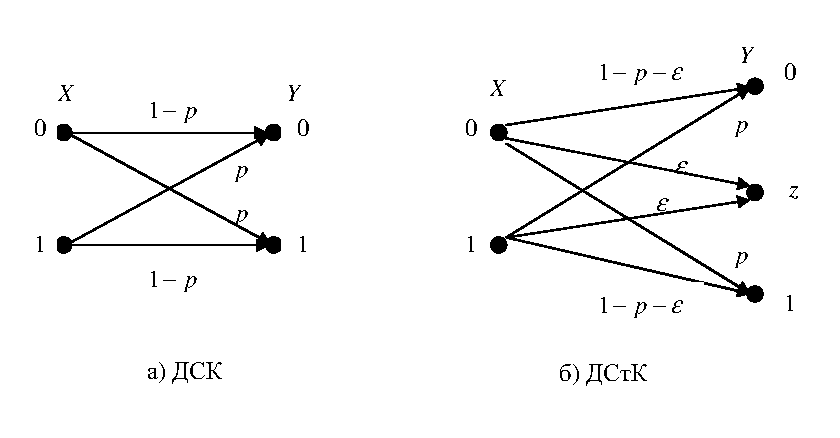
\includegraphics[width=1.0\textwidth]{fig5_2.eps}
%\centerline{\includegraphics[width=3.16in,height=4.02in]
\caption{Discrete stationary channels examples} \label{fig5_2}
\end{minipage}
\end{figure}

\end{itemize}
\end{frame}

\begin{frame}
\frametitle{Channel models}
\begin{itemize}
% \footnotesize {
% \small{
    \item Binary Symmetric Channel (BSC).
        $X = Y = \{0,1\}$,
        $p_{10} = p_{01} = p$, $p_{00} = p_{11} = 1 - p$.
        Transition probability matrix:
        \[
        P = \left[ {{\begin{array}{*{20}c}
         {1 - p} \hfill & p \hfill \\
         p \hfill & {1 - p} \hfill \\
        \end{array} }} \right].
        \]

    \pause \item
    Binary Symmetric Channel with Erasure (BSCE).
    \[
    P = \left[ {{\begin{array}{*{20}c}
     {1 - p - \varepsilon } \hfill \\
     p \hfill \\
    \end{array} }\mbox{ }{\begin{array}{*{20}c}
     \varepsilon \hfill \\
     \varepsilon \hfill \\
    \end{array} }\mbox{ }{\begin{array}{*{20}c}
     p \hfill \\
     {1 - p - \varepsilon } \hfill \\
    \end{array} }} \right].
    \]
    $X = {0,1}, Y = {0, 1, z}$, where $z$ is a special erasure symbol.

\end{itemize}
\end{frame}

% ------------------Mutual information---------------

\begin{frame}
\frametitle{Mutual information}
\begin{itemize}
% \footnotesize {
% \small{

    \item
    For a given $XY = \{(x,y),p(x,y)\}$ of ensembles $X$ and $Y$ calculate the information about $x \in X$ by $y \in Y$.

    \pause \item
    Mutual information:
    \begin{equation}
    \label{eq5_2} I(x;y) = I(x) - I(x\vert y).
    \end{equation}



\end{itemize}
\end{frame}


\begin{frame}
\frametitle{Mutual information}
\begin{itemize}
% \footnotesize {
% \small{
    \item
    \textit{Average mutual information} of $X$ and $Y$ is
    \[
    I(X;Y) = {\rm {\bf M}}\left[ {I(x;y)} \right].
    \]

    \pause \item
    Dependence between average mutual information and joint probability distribution:
    \begin{equation}
    \label{eq5_3} I(X;Y) = \sum\limits_{x \in X} {\sum\limits_{y \in
    Y} {p(x,y)\log \frac{p(y\vert x)}{p(y)}} } .
    \end{equation}

\end{itemize}
\end{frame}


\begin{frame}
\frametitle{Mutual information}
Properties of mutual information:

\begin{enumerate}
% \footnotesize {
% \small{

    \item[1]
    \begin{prop} \label{p5_1}
    Symmetricity: $I(x;y) = I(y;x)$.
    \end{prop}

    \pause \item[2]
    \begin{prop} \label{p5_2}
    If $x$ and $y$ are independent, $I(x,y) = 0$.
    \end{prop}

    \pause \item[3]
    \begin{prop} \label{p5_3}
    Symmetricity $I(X;Y) = I(Y;X)$\textbf{.}
    \end{prop}

    \pause \item[4]
    \begin{prop} \label{p5_4}
    Nonnegativity: $I(X;Y) \ge 0$.
    \end{prop}

    \pause \item[5]
    \begin{prop} \label{p5_5}
    Identity $I(X;Y) = 0$ holds iff  ensembles $X$ and $Y$ are independent.
    \end{prop}


\end{enumerate}
\end{frame}


\begin{frame}
\frametitle{Mutual information}
Properties of mutual information:

\begin{enumerate}
% \footnotesize {

    \item[6]
    \begin{prop} \label{p5_6}
    $I(X;Y) = H(X) - H(X\vert Y) = H(Y) - H(Y\vert X) =H(X) + H(Y) - H(XY).$
    \end{prop}


    \pause \item[7]
    \begin{prop} \label{p5_7}
    $I(X;Y) \le \min \left\{ {H(X),H(Y)} \right\}.$
    \end{prop}

    \pause \item[8]
    \begin{prop} \label{p5_8}
    $I(X;Y) \le \min \left\{ {\log \vert X\vert ,\log \vert Y\vert } \right\}.$
    \end{prop}

    \pause \item[9]
    \begin{prop}  \label{p5_9}
    Mutual information $I(X;Y)$ is a convex $ \cap $ function of probability distribution $p(x)$.
    \end{prop}

    \pause \item[10]
    \begin{prop}  \label{p5_10}
    Mutual information $I(X;Y)$ is a convex $ \cup $ function of conditional probabilities $p(y\vert x)$.
    \end{prop}


\end{enumerate}
\end{frame}

% ----------------Conditional average mutual information------

\begin{frame}
\frametitle{Conditional average mutual information.}
\begin{itemize}
% \footnotesize {
% \small{
    \item
    Consider $XYZ = \{(x,y,z),p(x,y,z)\}.$
    Fix $z \in Z$ and consider conditional probability distribution:
    $p(x,y\vert z) = \frac{p(x,y,z)}{p(z)}.$

    \item
    Average mutual information between $X$ and $Y$:
    $ I(X;Y\vert z) = \sum\limits_{x \in X} {\sum\limits_{y \in Y} {p(x,y\vert z)\log \frac{p(y\vert x,z)}{p(y\vert z)}} }.$

\end{itemize}
\end{frame}


\begin{frame}
\frametitle{Conditional average mutual information.}
\begin{itemize}
% \footnotesize {
% \small{
    \item
    Conditional average mutual information between $X$ and $Y$:

    $I(X;Y\vert Z) = {\rm {\bf M}}\left[ {I(X;Y\vert z} \right] = \sum\limits_{x \in X} {\sum\limits_{y \in Y} {\sum\limits_{z \in Z} {p(x,y,z)} \log \frac{p(y\vert x,z)}{p(y\vert z)}} }$

    \item
    Additional properties:
    $I(X;Y\vert Z) = H(Y\vert Z) - H(Y\vert XZ).$
    $I(X;YZ) &=& I(X;Y) + I(X;Z\vert Y)$
    $I(X;YZ) &=& I(X;Z) + I(X;Y\vert Z)$
\end{itemize}
\end{frame}

\begin{frame}
\frametitle{Conditional average mutual information.}
\begin{itemize}
% \footnotesize {
% \small{
    A special case of information processing system, which has 3 probability ensembles:
    \begin{figure}[ht]
    \begin{minipage}{1.0\linewidth}
    \includegraphics[width=1.0\textwidth]{fig5_3.eps}
    \caption{Information processing system} \label{fig5_3}
    \end{minipage}
    \end{figure}
\end{itemize}
\end{frame}

\begin{frame}
\frametitle{Conditional average mutual information.}
\begin{itemize}
% \footnotesize {
% \small{

    \begin{theorem}
    \label{th_inf_trans} Let $X$, $Y$, $Z$ be probability ensembles,
    which are formed by the information processing system at the previous slide. Then holds:
    \begin{eqnarray}
    \label{eq5_8} I(X;Y) &\ge& I(X;Z),\\
     \label{eq5_9} I(Y;Z) &\ge& I(X;Z).
    \end{eqnarray}
    \end{theorem}

\end{itemize}
\end{frame}


\begin{frame}
\frametitle{Conditional average mutual information.}
% \footnotesize {
% \small{

    \textbf{proof.} Use properties of conditional average mutual information:
    \begin{eqnarray}
    \label{eq5_10} I(X;YZ) &=& I(X;Y) + I(X;Z\vert Y), \\
    \label{eq5_11} I(X;YZ) &=& I(X;Z) + I(X;Y\vert Z).
    \end{eqnarray}
    $X$ and $Z$ are independent. If $Y$ is known, \\
    $I(X;Z\vert Y) = 0$.
    By equating the right sides of (\ref{eq5_10}) and
    (\ref{eq5_11}), we get
    \[
    I(X;Y) = I(X;Z) + I(X;Y\vert Z).
    \]
    Since the second term is non-negative, we obtain the inequality
    (\ref{eq5_8}). Similarly we can prove (\ref{eq5_9}).

\end{frame}



% ----------------Convexity of average mutual information---------

\begin{frame}
\frametitle{Convexity of average mutual information}
\begin{itemize}
% \footnotesize {
% \small{



\end{itemize}
\end{frame}

\end{document}